\section{Least-Squares Approximation}
\subsection{Lineare Least-Squares}
Ziel: Approximation von Messpunkten durch Minimieren einer Funktion, die die Abweichung in $y$
angibt (Residuen). Die Datenpunkte werden bei dieser Methode nicht mehr genau getroffen, ausserdem ist der Grad $m$ des Approximation-Polynoms meist massiv kleiner als die Anzahl der gegebenen Datenpunkte $N+1$.\\

Aus einer Menge von Basisfunktionen ${g_0,g_1,\ldots,g_m}$ mit $m \ll N$ und den Messungen $(x_0,y_0),(x_1,y_1),\ldots,(x_N,y_N)$ wird das überdeterminierte ($m<N$) Gleichungssystem aufgestellt und nach den unbekannten $a_i$ gelöst.
\[
    \overbrace{
    \begin{pmatrix}
        g_0(x_0) & g_1(x_0) & \ldots & g_m(x_0) \\
        \vdots & \vdots & \ddots & \vdots \\
        \vdots & \vdots & \ddots & \vdots \\
        g_0(x_N) & g_1(x_N) & \ldots & g_m(x_N)
    \end{pmatrix}}^{\text{Designmatrix } G}
    \cdot
    \begin{pmatrix}
        a_0 \\ \vdots \\ a_m
    \end{pmatrix}
    =
    \begin{pmatrix}
        y_0 \\ \vdots \\ \vdots \\ y_N
    \end{pmatrix}
    \qquad
    \Leftrightarrow
    \qquad
    G \cdot a = y
\]


\begin{minipage}[c]{12.5cm}
	\begin{tabular}{ll}
		Zu minimierende Fehlerfunktion:
		&$\boxed{\underbrace{S}_{Fehler}=\sum\limits_{i=0}^{N}{\big(y_i - \underbrace{\sum\limits_{j=0}^{m}{a_j g_j}}_{Modell}\big)^2} = \sum\limits_{i=0}^{N}{ r_i^2}}$\\
		Modellfunktion:
		&$\boxed{y=\sum\limits_{j=0}^{m}{a_j g_j}}\overset{Poly!}{=}\sum\limits_{j=0}^{m}{a_j x^j}$\\
		Abweichungen (Residuen):
		&$r_i=y_i-\sum\limits_{j=0}^{m}{a_j g_j}$
	\end{tabular}

	\subsubsection{Normalgleichung}

	Minimieren des quadratischen Fehlers mit "`Normalmatrix"' G (Designmatrix):
	$$\underbrace{\bm{G}^T \bm{G}}_{Normalmatrix}\cdot \bm{a} = \bm{G}^T \bm{y} \qquad \Rightarrow \qquad \bm{a}=(\bm{G}^T \bm{G})^{-1}\bm{G}^T \bm{y}$$
	$$\underbrace{\underbrace{\bm{G}^T}_{(m+1)\times(N+1)} \cdot \underbrace{\bm{G}}_{(N+1)\times(m+1)}}_{(m+1)\times(m+1)}\cdot
	  \underbrace{\bm{a}}_{(m+1)\times 1}=
	  \underbrace{\underbrace{\bm{G}^T}_{(m+1)\times(N+1)}\cdot\underbrace{\bm{y}}_{(N+1)\times 1}}_{(m+1)\times 1}$$
\end{minipage}
\hfill
\begin{minipage}[c]{6.5cm}
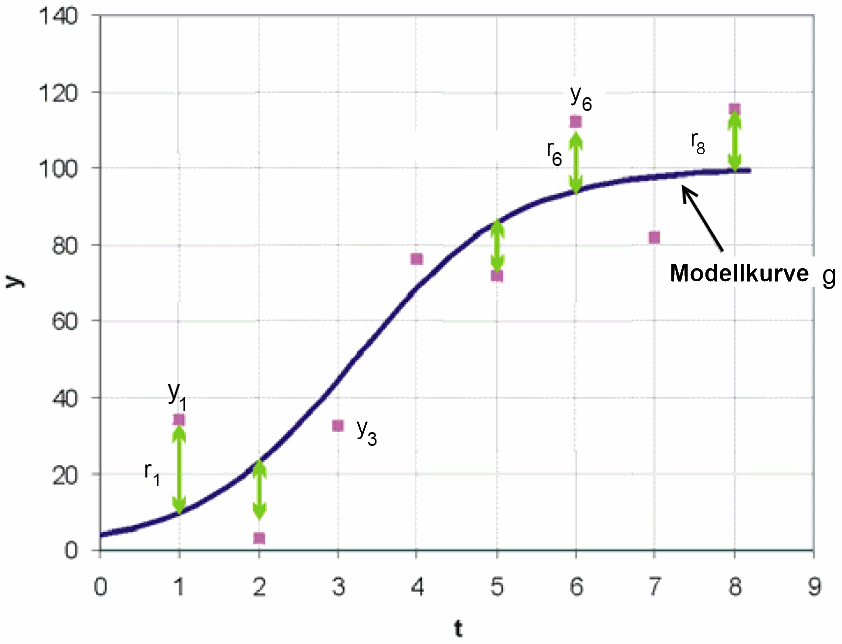
\includegraphics[width=\textwidth]{bilder/leastSquare}\\

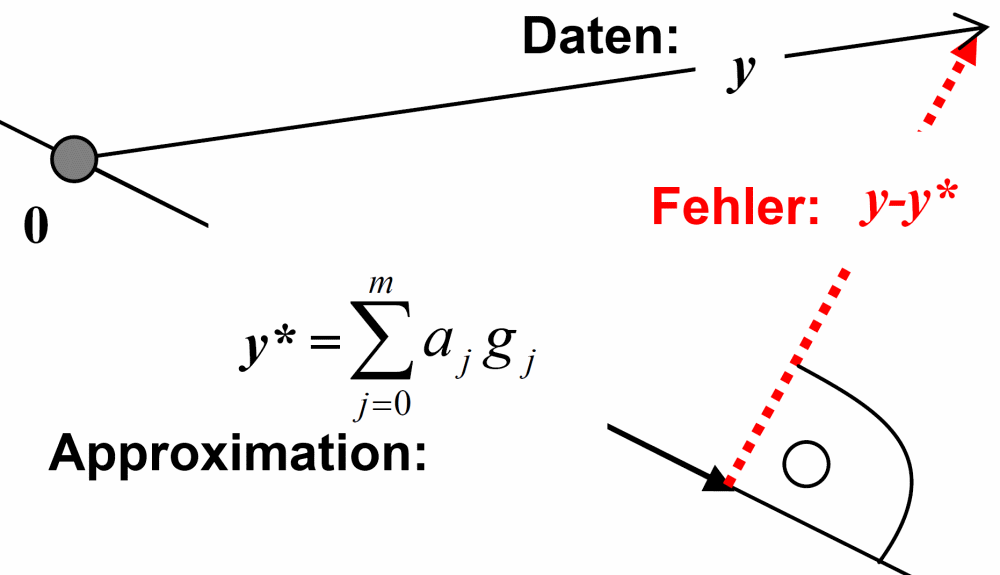
\includegraphics[width=1\textwidth,trim=-3cm 0cm 0cm 0cm]{bilder/leastSquareOrth}
\end{minipage}

Die symmetrische $(m+1)\times(m+1)$ Matrix $G^T \cdot G$ ist positiv definit wenn $g_i$ linear unabhängig sind.
Das neue Gleichungssystem ist regulär und hat eine eindeutige Lösung für die Koeffizienten $a_j$.
\[
    \overbrace{
    \begin{pmatrix}
        \langle g_0|,g_0|\rangle & \langle g_1|,g_0|\rangle & \ldots & \langle g_m|,g_0|\rangle \\
        \vdots & \vdots & \ddots & \vdots \\
        \langle g_0|,g_m|\rangle & \langle g_1|,g_m|\rangle & \ldots & \langle g_m|,g_m|\rangle
    \end{pmatrix}
    }^{G^T \cdot G}
    \cdot
    \begin{pmatrix}
        a_0 \\ \vdots \\ a_m
    \end{pmatrix}
    =
    \begin{pmatrix}
        \langle y|,g_0 |\rangle \\ \vdots \\ \vdots \\ \langle y|,g_m| \rangle
    \end{pmatrix}
\]

\subsubsection{QR-Zerlegung}
Eine quadratische $n \times n$ Matrix $Q$ ist orthogonal, falls $Q^T \cdot Q = Q \cdot Q^T = I$ bzw. $Q^T = Q^{-1}$.
Jede beliebige Matrix $G$ mit den Dimensionen $(N+1) \times (m+1)$ mit $N \geq m$ und Rang $m+1$ kann als
Produkt einer orthogonalen $(N+1)\times(N+1)$ Matrix $Q$ und einer $(N+1)\times(m+1)$ oberen Dreiecksmatrix $R$.

Aus dem Gleichungssystem $Ga| = y|$ wird dann $Ra|=Q^Ty|$, was einfacher lösbar ist\textsuperscript{Citation needed}.

\subsubsection{Singulärwertzerlegung (singular value decomposition, SVD)}
Jede Matrix $\bm G$ mit Dimensionen $(N+1) \times (m+1)$ kann so zerlegt werden:
$$\bm G = \bm U \bm D \bm V^T = \bm U \cdot \begin{bmatrix}
  d_{00} & 0      & \ldots & 0\\
  0      & d_{11} & \ldots & 0\\
  \vdots & \vdots & \ddots & 0\\
  0      & \ldots & 0      & d_{mm}\\
  0      & 0      & \ldots & 0\\
  \vdots & \vdots & \ddots & 0\\
  0      & 0      & \ldots & 0
\end{bmatrix} \cdot \bm V^T$$
$\bm D$ ($(N+1) \times (m+1)$) ist die zentrale Diagonalmatrix mit Singulärwerten,
$\bm U$ ($(N+1) \times (N+1)$) und $\bm V$ ($(m+1) \times (m+1)$) sind orthogonale und quadratische
Matrizen (d.h. u.a. $\bm U^T=\bm U^{-1}$).\\

Die Zerlegung an sich wird hier nicht weiter ausgeführt, diese kann anderswo nachgeschlagen werden.
SVD kann gebraucht werden, um Gleichungssystem zu lösen (wie hier), um Eigenvektoren und Eigenwerte
sowie die Inverse zu berechnen.

Aus $Ga|=y|$ wird $UDV^T a|=y|$. Dies lässt sich auflösen zu
\[
    a| = V D^{-1}U^T \cdot y|
\]

\subsubsection{Monomiale} \label{sssec:ls_monomiale}
Mit
$g = a_0 \underbrace{1}_{g_0} + a_1 \underbrace{x}_{g_1} + a_2 \underbrace{x^2}_{g_2} +\ldots + a_m \underbrace{x^m}_{g_2}$
wird die Designmatrix zu:
\[G \underbrace{=}_{\text{When Monomials}}
\begin{bmatrix}
  1 & x_0 & x_0^2  & \ldots & x_0^m\\
  1 & x_1 & x_1^2  & \ldots & x_1^m\\
  \vdots  & \vdots & \vdots  & \ddots & \vdots\\
  1 & x_N & x_N^2  & \ldots & x_N^m\\
\end{bmatrix}\]


\subsubsection{Gleichförmige Argumente\quad (Orthogonalitäts-Eigenschaften)} \label{sssec:ls_orthogonal}
Mit gleichförmigen Elementen $x_i - x_j = (j-i) h$ für alle $i,j$ $\rightarrow$ $\{x_0...x_N\} = \{x_0 + t \cdot h\}_{t=0...N}$ und \textbf{orthogonalen Polynomen} kann
$G G^T$ diagonalisiert und so die Gleichungen rechnerisch einfacher gelöst werden.

$$\boxed{p_{k,N}(t) = \sum_{i=0}^k (-1)^i \binom{k}{i} \binom{k+i}{i} \frac{t^{(i)}}{N^{(i)}}=
1+\sum_{i=1}^k (-1)^i \binom{k}{i} \binom{k+i}{i} \frac{t(t-1)(t-2)\ldots(t-i+1)}{N(N-1)(N-2)\ldots(N-i+1)} \qquad (k = 1,\ldots,N)}$$
mit $t=\frac{x-x_0}{h} \qquad \binom{k}{i}=\frac{k!}{i!(k-i)!}=nCr(k,i)$\\
$p_{k,N}$ kann jetzt als $g_{k}$ in die Designmatrix eingesetzt werden und das Produkt $G^T G$ wird
zu einer $(m+1)\times(m+1)$ Diagonalmatrix. Schlussendlich kann $a$ über die bekannte Formel
$G^T G a = G^T y$ berechnet werden.\\

\textbf{Beispiel:}
$$\bm{x}=
	   \begin{bmatrix}
			3&4&5&6&7
	   \end{bmatrix}\qquad \Rightarrow\qquad \bm{t}=\bm{x}-3=
	   \begin{bmatrix}
	   		0&1&2&3&4
	   \end{bmatrix}$$
$$\Rightarrow P_0(x)=1 \qquad P_1(x)= 1-\frac{x-3}{2}\qquad P_2(x)=1-\frac{2\cdot 3 (x-3)}{4}+\frac{1 \cdot 3 (x-3)(x-3 -1)}{4 \cdot 3} = 1-\frac{3x-9}{2}+\frac 12 (x-4)(x-3)???$$
$$\overset{\hspace{0.6cm} P_0 \hspace{0.5cm} P_1 \hspace{0.6cm} P_2}{\bm{G} = \begin{bmatrix}
  1 & 1 	& 1\\
  1 & 1/2 	& -1/2\\
  1 & 0	  	& -1\\
  1 & -1/2 	& -1/2\\
  1 & -1 	& 1\\
\end{bmatrix}}\qquad \Rightarrow\qquad
\bm{G}^T\bm{G}=\begin{bmatrix}
 \| P_0\|^2 	& 0 	& 0\\
  0 		& \|P_1\|^2 	& 0\\
  0 		& 0	  	&\|P_2\|^2\\
\end{bmatrix}
= \begin{bmatrix}
  5 & 0 & 0 \\
  0 & \frac52 & 0\\
  0 & 0 & \frac{7} {2}\\
\end{bmatrix}
$$

\newpage
\subsubsection{Chebyshev Orthogonale Polynome} \label{sssec:chebyshev_polynom}
\textbf{Idee}: Approximation eines kontinuierlichen Polynoms durch Chebyshev-Polynome.

\textbf{Definition}\\
Chebyshev Polynome sind definiert als $\boxed{T_n(x) = \cos(n \arccos(x))}$ mit $(n = 0,1,\ldots)$ und $(-1 \leq x \leq 1)$. Dieses
Polynom bewirkt eine Häufung der Messwerte in den Randbereichen. Die
ersten paar Polynome $T_n$ sowie deren Umformungen nach $x$:\\
\begin{tabular}{ll}
  $T_0 = 1$ & $x^0 = 1 = T_0$ \\
  $T_1 = x$ & $x^1 = x = T_1$ \\
  $T_2 = 2x^2 -1$ & $x^2 = \frac12 T_2 + \frac12 T_0$ \\
  $T_3 = 4x^3 - 3x$ & $x^3 = \frac14 T_3 + \frac34 T_1$\\
  $T_4 = 8x^4 -8x^2 + 1$ & $x^4 = \frac18 T_4 + \frac12 T_2 + \frac38 T_0$\\
  $T_5 = 16x^5 - 20x^3 + 5x$ & $x^5 = \frac{1}{16} T_5 + \frac{5}{16} T_3 + \frac58 T_1$\\
\end{tabular}

Weitere Chebyshev Polynome können mit der Rekursionsformel $T_{n+1}(x) = 2x T_n(x)-T_{n-1}\;(n\geq2)$
mit Initialbedingungen $T_1(x)=x,\;T_0(x)=1$ berechnet werden.\\

\textbf{Eigenschaften: }
\begin{itemize}
  \item Die maximale Amplitude des Chebyshev-Polynoms ist $\frac{1}{2^n}$ (max Amplitude des Fehlerterms).
  \item Amplitude: $T_n(x) \in [-1,+1]$
  \item Nullstellen: $T_n(x)=0 \Leftrightarrow x=\cos(\frac{2i+1}{2n}\pi)\qquad i=0,1,\ldots,n-1$ (Diese Nullstellen sind die Chebyshev-Knoten)
  \item $T_n(x)= \pm 1 \Leftrightarrow x=\cos(\frac{i\pi}{n}) \; (i=0,1,\ldots,n)$
\end{itemize}

\begin{minipage}{9cm}
  \textbf{Rezept}\\
  Chebyshev Polynome können nur benutzt werden, wenn \textbf{$x$ mit Chebyshev-Abständen}
  $x_i=\cos(\frac{2i+1}{2n}\pi)\;(i=0,1,\ldots,n-1)$ und nicht
  mit gleichverteilten Abständen gewonnen wurden.

  Ziel: $y(t) = p_N(t)$ (Polynom, definiert in $[a,b]$) mit Chebyshev-Polynomen des Grades
  $m$ approximieren.
  \begin{enumerate}
    \item $y(t)$ auf das Standardintervall $[-1,1]$ normieren (affine Transformation)
    $t = a + \frac{b-a}{2} (x+1)$.
    \item $y(x)$ aus $T_n$ zusammensetzen
    \item $y(x)$ auf Grad $m$ kürzen (truncate): $y_m(x)$
    \item Zurücktransformieren: $x = 2\frac{t-a}{b-a}-1$
    \item $T_n$ in $y_m$ einsetzen (siehe Tabelle oben)
    \item Fehlerabschätzung für truncate Methode:\\
      $\max_{t} |y(t) - y_m(t)|$ (Abgeschnittener Teil)
  \end{enumerate}
\end{minipage}
\hspace{1cm}
\begin{minipage}{9cm}
  \textbf{Beispiel}\\
  Gesucht: Approximation $y(t)=t^3$ mit Grad $m=2$ für Intervall $(a,b) = (0,1)$
  \begin{enumerate}
  	\item Transformation mit $t = \frac{x+1}{2}$:\\
  	  $y(x) = \left( \frac{x+1}{2} \right)^3 = \frac18 (x^3 + 3x^2 + 3x + 1)$
  	\item Mit Tabelle erweitern:\\
  	$y(x) = \frac18 \left( \frac{T_3(x) + 3 T_1(x)}{4} + 3 \frac{T_2(x) + T_0}{2} + 3T_1(x) + T_0(x) \right)$\\
  	$=\frac{1}{32}T_3(x) + \frac{3}{16}T_2(x) + \frac{15}{32} T_1(x) + \frac{5}{16}T_0(x)$
  	\item Kürzen auf Grad $m=2$:\\
  	  $y(x) \approx \frac{3}{16}T_2(x) + \frac{15}{32}T_1(x) + \frac{5}{16}T_0(x)$
  	\item Zurücktransformieren mit $x = 2t-1$:\\
  	  $y(t) \approx \frac{3}{16}T_2(2t-1) + \frac{15}{32}T_1(2t-1) + \frac{5}{16}T_0(2t-1)$
  	\item $T_n(2t-1)$ ersetzen:\\
      $y(t) \approx \frac{3}{16} (2(2t-1)^2-1) + \frac{15}{32}(2t-1) + \frac{5}{16}$
    \item Fehlerabschätzung:\\
      $\max_t \left| \frac{1}{32}T_3(2t-1) \right|$
  \end{enumerate}
\end{minipage}

\newpage

Die \textbf{Designmatrix} sieht so aus:
$$G \underbrace{=}_{\text{When Chebyshev}}
\begin{bmatrix}
  T_0(x_0) = 1 & T_1(x_0) = x_0 & \ldots & T_m(x_0) \\
  T_0(x_1) = 1 & T_1(x_1) = x_1 & \ldots & T_m(x_1)\\
  \vdots & \vdots  & \ddots & \vdots\\
  T_0(x_N) = 1 & T_1(x_N) =x_N & \ldots & T_m(x_N)\\
\end{bmatrix}_{N \times m}$$

Damit wird $G^T G$ zu:
$$G^T G \underbrace{=}_{\text{When Chebyshev}}
\begin{bmatrix}
  N+1 & 0 & \ldots & 0 \\
  0   & \frac{N+1}{2} & \ldots & 0\\
  \vdots  & \vdots & \ddots & \vdots\\
  0   & 0 & \ldots & \frac{N+1}{2}\\
\end{bmatrix}_{m \times m}$$

und $(G^T G)^{-1} G^T$ zu:

$$(G^T G)^{-1} G^T \underbrace{=}_{\text{When Chebyshev}}
\begin{bmatrix}
  \frac{1}{N+1} T_0(x_0) = \frac{1}{N+1} & \frac{1}{N+1} T_0(x_1) = \frac{1}{N+1} & \ldots & \frac{1}{N+1} T_0(x_N) = \frac{1}{N+1} \\
  \frac{2}{N+1} T_1(x_0) = \frac{2}{N+1} x_0 & \frac{2}{N+1} T_1(x_1) = \frac{2}{N+1} x_1 & \ldots & \frac{2}{N+1} T_1(x_N) = \frac{2}{N+1}x_N\\
  \vdots & \vdots  & \ddots & \vdots\\
  \frac{2}{N+1} T_m(x_0) & \frac{2}{N+1} T_m(x_1) & \ldots & \frac{2}{N+1} T_m(x_N)\\
\end{bmatrix}_{m \times N}$$

\subsubsection{Diskrete Least-Squares Chebyshev Approximation}
Folgt aus $a=(G^T G)^{-1} G^T y$ für $x_i=\cos(\frac{2i+1}{2(N+1)}\pi)\;(i=0,1,\ldots,N)$:
$$p(x) = \sum_{j=0}^m a_j T_j(x) \quad \text{wobei} \quad
a_j = \begin{cases}
  \frac{1}{N+1} \sum_{i=0}^N y(x_i) & j = 0\\
  \frac{2}{N+1} \sum_{i=0}^N T_j(x_i) y(x_i) & j > 0
\end{cases}$$

\subsubsection{Kontinuierliche Least-Squares}
Für kontinuierliche Funktionen, die \textbf{keine Polynome} sind (!) kann auch die kontinuierliche Version
verwendet werden.\\
S: zu minimierende Fehlerfunktion, w: Gewicht mit  ($-1\leq x \leq1$)
\[
	S = \int\limits_{-1}^1 (y(x) - p(x))^2 \cdot w(x) \cdot \mathrm{d}x
\]

\textbf{Kontinuierliche Least-Squares Chebyshev Approximation}\\
 Das Gewicht wird besonders auf den Rand gelegt (wie bei Chebyshev üblich). ($w(x) = \frac{1}{\sqrt{1-x^2}}$)
$$p(x) = \sum_{j=0}^m a_j T_j(x) \quad \text{wobei} \quad
a_j = \begin{cases}
  \frac{1}{\pi} \int_{-1}^1 \frac{y(x)}{\sqrt{1-x^2}} dx & j = 0\\
  \frac{2}{\pi} \int_{-1}^1 \frac{y(x) T_j(x)}{\sqrt{1-x^2}} dx & j > 0
\end{cases}$$

\textbf{Kontinuierliche Least-Squares Legendre Approximtion:}\\
Hier bei wird das Gewicht $w(t) = 1$ gesetzt.\\

Legendre Polynome:
\[
  P_n(x) = \frac{1}{2^n n!} \cdot \frac{\mathrm{d}^n}{\mathrm{d}x^n}(x^2-1)^n \qquad \qquad P_0(x) = 1 \qquad P_1(x) = x \qquad P_2(x) = \frac{1}{2}(3x^2-1)
\]
\[
	  P_3(x) = \frac{1}{2}(5x^3 - 3x) \qquad P_4(x) = \frac{1}{8}(35x^4-30x^2+3) \qquad P_5(x) = \frac{1}{8}(63x^5-70x^3+15x)
\]
\[
	  1 = P_0(x)  \quad x = P_1(x) \quad x^2 = \frac{2P_2(x) + P_0(x)}{3} \quad x^3 = \frac{2P_3(x)+ 3 P_1(x)}{5} \quad x^4 = \frac{8P_4(x) + 20 P_2(x) + 7 P_0(x)}{35} 
\]

Koeffizenten:
$$
	p(x) = \sum_{j=0}^m a_j P_j(x) \quad \text{wobei} \quad
	a_j = \frac{2j+1}{2} \cdot \int\limits_{-1}^{1}y(x) P_j(x) \cdot \mathrm{d}x \qquad (j=0,1,...,m)
$$

\subsection{Multi-Variate Lineare Least Squares Approximation}
Multi-Variate Least Square Probleme werden genau gleich wie die Uni-Variaten Least Square Probleme gelöst (selbe Methoden)! Die Variable $x$ ist keine Zahl mehr, sondern ein Vector mit $d$ Dimensionen!

\textbf{Basisgewinnung:}
Die Basen werden mittel Tensorenprodukt aus Uni-Variaten Basen berechenet (Alle mit allen Multiplizieren (d-Basen in d-Variabeln)).

\[
	\sum\limits_{j_1=0}^{m_1} \sum\limits_{j_2=0}^{m_2} ... \sum\limits_{j_d=0}^{m_d} a_{j_1,j_2,...,j_d} \cdot g_{j_1}(x^{(1)}) g_{j_2}(x^{(2)}) \cdot \cdot ... \cdot g_{j_d}(x^{(d)})
\]

\paragraph{Beispiele}
\begin{align*}
    &\text{Basis 3. Grad:} &&
    \{ 1,x,y, \; x^2,2xy,y^2, \; x^3,3x^2y,3xy^2,y^3 \} \\
    &\text{Basis 4. Grad:} &&
    \{ 1,x,y, \; x^2,2xy,y^2, \; x^3,3x^2y,3xy^2,y^3, \; x^4,4x^3y,6x^2y^2,4xy^3,y^4\} \\
\end{align*}

\subsection{Legendre Polynome}
Die Legendre $P$-Polynome werden durch die Rodriguez' Formel bestimmt
\[
    P_n(x) = \frac{1}{2^n n!} \cdot \frac{d^n}{dx^n} \left( x^2-1 \right)^n
\]
\[
    P_0(x) = 1 \qquad P_1(x) = x \qquad P_2(x) = \frac{1}{2}(3x^2-1) \qquad
    P_3(x) = \frac{1}{2}(5x^3-3x) \quad P_4(x) = \frac{1}{8}(35x^4-30x^2+3)
\]
